%---------------------------------------------------------------------
\chapter{Observability and Evaluation}\label{ch:eval}
%---------------------------------------------------------------------
\section{Tracing and Observability}\label{sec:trace}
Every agent step is recorded as a typed event (kinds include \texttt{PLAN}, \texttt{OCR}, \texttt{THINK}, \texttt{TOOL}, \texttt{MATCH}, \texttt{RAG}, \texttt{GRADE}, \texttt{REQUERY}, \texttt{ABSTAIN}, \texttt{BUILD}, \texttt{VERIFY}, \texttt{HUMAN}, \texttt{LLM}, \texttt{GUARD}, \texttt{LIMIT}). The events go to three sinks: a coloured console log, a JSONL and HTML file per case that is always written, and a Langfuse trace when a server is reachable. The case identifier is the Langfuse session, so the separate traces that a pause and resume produces are grouped. All sinks receive masked data. A warning level marks events that are rejections or send-backs, which makes the interesting parts of a run visible at a glance.

Figure~\ref{fig:lf-a} shows the Langfuse trace of the worked example (Section~4.5). The trace is a tree: one span per graph node, events under it.

\begin{figure}[t]
\centering
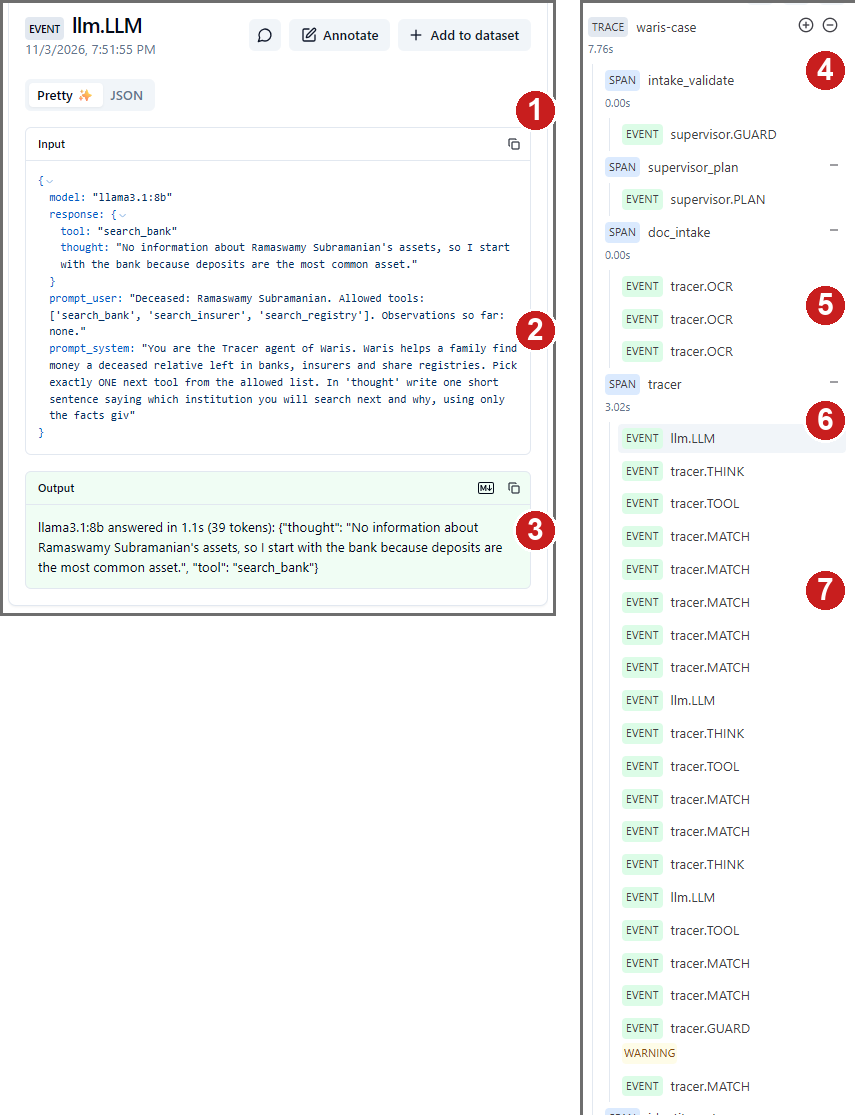
\includegraphics[width=0.66\linewidth]{figures/fig_langfuse_a.png}
\caption[Langfuse trace of the worked example (first half)]{Langfuse trace of the worked example, first half. (1) An \texttt{llm.LLM} event; (2) its input: model, system prompt, user prompt and the parsed response; (3) the output text with the 1.1\,s duration and 39 tokens; (4) the trace root \texttt{waris-case}, 7.76\,s in total; (5) the three OCR events of \texttt{doc\_intake}; (6) the model call that chose the first tool; (7) one \texttt{tracer.MATCH} event for each record scored.}
\label{fig:lf-a}
\end{figure}

The second half of the trace, which shows the grading, the abstention and the Verifier send-back, is reproduced in Figure~\ref{fig:lf-b} of Appendix~C.


The traces serve debugging and audit as well as evidence. The grade event of Figure~\ref{fig:lf-b}, for example, states the stage at which a rule was rejected and the reason, which is what a reviewer needs in order to check an abstention.

\section{Evaluation Dataset}\label{sec:dataset}
The benchmark is the synthetic set described in Section~\ref{sec:data}; its construction is in Section~6.2. Table~\ref{tab:dataset} gives its composition; the distribution of the true statuses is given after the list. Three sets are used.

\begin{itemize}[leftmargin=*,itemsep=2pt]
\item \textbf{Main set}: 60 families. The 40 development families were used to build and tune; the 20 held-out test families were not used for decisions. Headline numbers are for the test families, with the development and all-60 figures reported alongside.
\item \textbf{Fresh-seed set}: 60 further families generated with a different seed and folder after the decision code was frozen, run once per variant. It checks that the system was not fitted to particular names.
\item \textbf{Stress set}: 12 medium families in which the family holds every required document except the name affidavit and an initials variant is present. It isolates what the Verifier contributes.
\end{itemize}

\begin{table}[H]
\centering\small\setstretch{1.0}
\caption{Composition of the main benchmark.}\label{tab:dataset}
\renewcommand{\arraystretch}{1.1}
\begin{tabular}{@{}lrrrr@{}}
\toprule
\textbf{Split} & \textbf{Easy} & \textbf{Medium} & \textbf{Hard} & \textbf{Families / assets} \\ \midrule
Development & 10 & 17 & 13 & 40 / 50 \\
Held-out test & 5 & 8 & 7 & 20 / 26 \\
\textbf{Total} & 15 & 25 & 20 & 60 / 76 \\ \bottomrule
\end{tabular}
\end{table}

Of the 76 true assets, 62 are \textsc{missing\_items} (36 bank deposits, 13 policies, 13 holdings), 6 are \textsc{ready} (3 deposits, 3 holdings) and 8 are \textsc{needs\_human\_review} (3, 3 and 2). The classes are imbalanced: \textsc{missing\_items} is the common outcome, which is realistic, since families rarely hold every document. This is why we report checklist-level metrics and per-case metrics in addition to status accuracy, and why the stress set exists.

\section{Metrics and the Judge}\label{sec:judge}
All metrics except the letter judge are computed against the generator's answer key.

\begin{itemize}[leftmargin=*,itemsep=2pt]
\item \textbf{Asset recall} $=|\text{found}\cap\text{true}|/|\text{true}|$; an abstained asset counts as found.
\item \textbf{Wrong-person matches} $=$ number of claimed records that are not true assets (target 0).
\item \textbf{Status accuracy} $=$ assets with the correct status / true assets.
\item \textbf{Checklist precision and recall} (micro-averaged over assets) $P=\sum|\hat D\cap D|/\sum|\hat D|$, $R=\sum|\hat D\cap D|/\sum|D|$, and $F_1=2PR/(P+R)$, where $D$ is the required document set of the key and $\hat D$ the predicted set; documents listed for a wrongly claimed asset count as false positives.
\item \textbf{Citation coverage} $=$ checklist items with an existing rule identifier / all items.
\item \textbf{Abstention correct} $=$ the set of assets marked \textsc{needs\_human\_review} equals the key's set (per case).
\item \textbf{Cases fully correct} $=$ share of runs with correct statuses and abstentions, an exact checklist and no wrong-person claim.
\item \textbf{Family-question precision and recall} $=$ questions asked versus the key's expected questions.
\item \textbf{Extraction accuracy} $=$ fields correctly read from the documents / fields in the documents (420 fields in the 60 families).
\item \textbf{Letter quality}: five yes/no criteria (right deceased, claimant and asset; the enclosed and still-to-follow lists match the true checklist; formal tone; nothing invented; a clear request), scored 0--5. Primary scoring is by a deterministic reference checker; a language-model judge (Llama 3.1 8B, one question per criterion) is scored alongside.
\end{itemize}

\paragraph{Judge validation.} The judge is the same model family that drafts the opening paragraph of the letters, so it cannot be trusted by default. We built a validation set of 33 letters: 12 genuine letters and 21 deliberately damaged ones (a document dropped, a wrong name, an invented amount, an invented date, an informal tone), and compared the judge's 165 criterion marks with the deterministic reference marks. Agreement was 89.1\% and Cohen's kappa $\kappa=0.56$ \cite{cohen1960kappa}, which is moderate. Per criterion: formal tone and clear request $\kappa=1.0$; nothing invented $\kappa=0.66$; documents match $\kappa=0.37$; asset and claimant $\kappa=0$ (the criterion has almost no negative marks in the set, which makes kappa uninformative, although the raw agreement is 84.8\%). We therefore use the reference checker as the primary letter metric and report the judge as a secondary signal. \emph{The judge was validated against a deterministic checker, not against human labels}; the template for the team's own marks of 15 letters exists in the repository but has not been filled in, so we make no claim about agreement with people.

\section{Baselines and Variants}
Five variants were run on every family. The \emph{one-pass baseline} uses the same tools (OCR, portal search, rule retrieval, letter writer) but none of the agentic decisions: it takes the single best name match per institution, trusts the single most similar rule, asks the model once per asset to turn the rule into a checklist, and has no Verifier, no human question and no document-conflict detection. The other variants remove one component of the full system.

The variants are: full Waris; the baseline; \emph{no grading}, in which the Rules Expert trusts the top-1 rule; \emph{no Verifier}, which passes every pack; and \emph{LLM off}, with a fixed tool order and template letters.

Each variant was run three times per family (reps 0, 1 and 2, with model temperature 0, 0.3 and 0.7 and seeds 0, 1 and 2). The family is simulated by a scripted oracle that answers identity questions from the answer key; this is disclosed in every result file. Where a document is unreadable by design, the harness types the true value, as a family would on the confirm screen; there were 10 such fields.

\section{Results}
Table~\ref{tab:main} gives the headline results on the 20 held-out test families (26 assets); Figure~\ref{fig:bars} plots the three main metrics. The spread over the three repetitions is zero for every metric except the run time. We report this plainly: the model is used only for the choice of portal and for letter wording, and the decisions that determine the metrics are made by fixed code, so changing the temperature and seed changed which portal was searched first, not the outcome. The standard deviation of the run time was below 0.1\,s.

\begin{table}[H]
\centering\footnotesize\setstretch{1.0}
\caption[Results on the held-out test families]{Results on the 20 held-out test families (3 repetitions; mean, with standard deviation over repetitions in brackets where non-zero).}\label{tab:main}
\renewcommand{\arraystretch}{1.1}
\begin{tabularx}{\linewidth}{@{}p{3.6cm}rrrrr@{}}
\toprule
\textbf{Metric} & \textbf{Baseline} & \textbf{$-$Grading} & \textbf{$-$Verifier} & \textbf{LLM off} & \textbf{Full} \\ \midrule
Status accuracy & 73.1\% & 92.3\% & 100\% & 100\% & \textbf{100\%} \\
Checklist F1 & 61.7\% & 69.0\% & 97.1\% & 100\% & \textbf{100\%} \\
Checklist precision & 64.1\% & 75.6\% & 100\% & 100\% & 100\% \\
Checklist recall & 59.5\% & 63.6\% & 94.4\% & 100\% & 100\% \\
Asset recall & 80.8\% & 100\% & 100\% & 100\% & 100\% \\
Wrong-person matches & 3 & 0 & 0 & 0 & \textbf{0} \\
Abstention correct & 85.0\% & 90.0\% & 100\% & 100\% & 100\% \\
Citation coverage & 100\% & 100\% & 100\% & 100\% & 100\% \\
Cases fully correct & 25.0\% & 35.0\% & 70.0\% & 100\% & \textbf{100\%} \\
Family-question recall & 0\% & 100\% & 100\% & 100\% & 100\% \\
Model calls / case & 2.4 & 2.7 & 2.6 & 0 & 2.6 \\
Seconds / case & 2.9 (0.0) & 3.4 (0.0) & 3.3 (0.0) & 0.0 & 3.3 (0.1) \\ \bottomrule
\end{tabularx}
\end{table}

\begin{figure}[t]
\centering
\begin{tikzpicture}
\begin{axis}[ybar, width=\linewidth, height=6.2cm, bar width=9pt, ymin=0, ymax=112, ylabel={percent},
  symbolic x coords={Baseline,{$-$Grading},{$-$Verifier},{LLM off},Full}, xtick=data, enlarge x limits=0.12,
  legend style={at={(0.5,1.03)},anchor=south,legend columns=3,font=\footnotesize},
  nodes near coords, every node near coord/.append style={font=\tiny, rotate=90, anchor=west},
  tick label style={font=\footnotesize}]
\addplot[fill=bmsblue!85] coordinates {(Baseline,73.1) ({$-$Grading},92.3) ({$-$Verifier},100) ({LLM off},100) (Full,100)};
\addplot[fill=orange!80] coordinates {(Baseline,61.7) ({$-$Grading},69.0) ({$-$Verifier},97.1) ({LLM off},100) (Full,100)};
\addplot[fill=ForestGreen!75] coordinates {(Baseline,25) ({$-$Grading},35) ({$-$Verifier},70) ({LLM off},100) (Full,100)};
\legend{Status accuracy, Checklist F1, Cases fully correct}
\end{axis}
\end{tikzpicture}
\caption[Status accuracy, F1 and fully correct cases (test families)]{Held-out test families: status accuracy, checklist F1 and fully correct cases for the five variants (3 repetitions, identical in each).}
\label{fig:bars}
\end{figure}

\paragraph{Larger sets.} Table~\ref{tab:sets} repeats the key comparisons on all 60 families, on the fresh-seed set and on the stress set. The picture is the same. The baseline claims a stranger's record 8 times over the 60 main families (24 wrong-person claims in the 3 repetitions) and 15 times over the 60 fresh families; the full system never does. On the stress set the status accuracy without the Verifier is 0\% against 100\% with it, because every one of the 12 families holds everything except the name affidavit that the first rule lookup does not return.

\begin{table}[H]
\centering\small\setstretch{1.0}
\caption[Key results on the larger sets]{Key results on the larger sets (status accuracy / checklist F1 / wrong-person claims).}\label{tab:sets}
\renewcommand{\arraystretch}{1.1}
\begin{tabularx}{\linewidth}{@{}p{3.3cm}XXX@{}}
\toprule
\textbf{Variant} & \textbf{Main, all 60 (3 reps)} & \textbf{Fresh-seed 60 (1 rep)} & \textbf{Stress 12 (1 rep)} \\ \midrule
One-pass baseline & 72.4\% / 60.9\% / 8 & 71.1\% / 57.8\% / 15 & 66.7\% / 60.2\% / 0 \\
$-$Grading & 90.8\% / 68.8\% / 0 & 90.8\% / 68.8\% / 0 & 100\% / 74.8\% / 0 \\
$-$Verifier & 100\% / 96.4\% / 0 & 100\% / 96.4\% / 0 & \textbf{0\%} / 89.7\% / 0 \\
LLM off & 100\% / 100\% / 0 & 100\% / 100\% / 0 & 100\% / 100\% / 0 \\
Full Waris & \textbf{100\% / 100\% / 0} & \textbf{100\% / 100\% / 0} & \textbf{100\% / 100\% / 0} \\ \bottomrule
\end{tabularx}
\end{table}

\paragraph{By difficulty.} The baseline's share of fully correct cases falls from 46.7\% on easy families to 16.0\% on medium and 10.0\% on hard ones, and all 24 of its wrong-person claims occur on hard families; the full system is at 100\% on all three (Figure~\ref{fig:diff}).

\paragraph{Letters.} Scored by the deterministic checker, the letters of the full system average 4.76 of 5 criteria, those of the baseline 3.76, the no-grading variant 4.08 and the no-Verifier variant 4.46. The judge ranks the variants in the same order for these four (4.01, 3.43, 3.58 and 3.79) but scores every variant lower than the checker, mainly because it marks letters as containing invented content more often than the checker does (Section~\ref{sec:judge}). The letters of the LLM-off variant are template-only and score 4.76 on the checker, equal to the full system; the judge scores them higher (4.18 against 4.01), so the model-written paragraph does not improve letter quality on these metrics.

\paragraph{Extraction.} The OCR engine read all 420 fields of the 60 families correctly on the documents that are meant to be readable; the 10 fields of blurred or faded documents were typed, by design.

\section{Error Analysis}
The full system made no error on the main set (the failure report of repetition 0 lists no imperfect run), so the analysis concerns the baseline and the ablations, which shows what each component prevents, and the errors found and fixed while the system was being built. Counts below are for repetition 0 over the 60 families (76 assets); the other repetitions are identical.

\begin{table}[H]
\centering\footnotesize\setstretch{1.0}
\caption[Failure modes of the variants]{Failure modes of the variants, with counts, an example and the component that prevents them.}\label{tab:errors}
\renewcommand{\arraystretch}{1.1}
\begin{tabularx}{\linewidth}{@{}p{1.7cm}p{3.1cm}p{3.6cm}X@{}}
\toprule
\textbf{Variant} & \textbf{Failure (count)} & \textbf{Example} & \textbf{Cause and what prevents it} \\ \midrule
Baseline & Wrong-person claims (8) & namesake families (7 of 8) & Best name match taken without checking date of birth and city. \emph{Identity policy.} \\
Baseline & True assets missed (12 of 76) & name variants, several accounts & Only one record per institution is taken. \emph{Scoring all records, aliases.} \\
Baseline & Wrong status where found (9) & 6 should be \textsc{needs\_human\_review}, 3 \textsc{ready} & No abstention; wrong rule trusted. \emph{Grading, abstention.} \\
Baseline & Checklist errors (121 missing, 77 extra documents) & legal-heir families: 5.3\% fully correct against 57.9\% for nominee families & Most similar rule trusted. \emph{Grading.} \\
$-$Grading & Wrong status (7 assets in 6 cases) & legal-heir and no-rule families & Nominee rule accepted for a legal heir; no abstention when no rule exists. \emph{Grading, re-query.} \\
$-$Grading & Checklist errors (124 missing, 62 extra) & as above & Wrong rule gives wrong documents. \\
$-$Verifier & Missing name affidavit (23 cases, 23 documents) & initials, spelling, maiden-name and order variants & The first rule lookup does not return the name-variation rule. \emph{V3 send-back.} \\ \bottomrule
\end{tabularx}
\end{table}

\paragraph{Errors found during development and their fixes.} (i)~A family claiming under the maiden name of the deceased was missed because only the certificate name was searched; the Tracer now searches every name the family knows. (ii)~The judge, when asked whether a letter was correct, accepted a letter that said an asset had ``matured on'' a date; the letter validator was tightened to forbid maturity, amounts and entitlement, and the judge was changed to five narrow yes/no questions. (iii)~Some synthetic families had lookalike records of other families that happened to satisfy the identity policy; the generator now keeps names unique, draws namesake cities from a separate list and checks every portal row against the policy. (iv)~OCR misreads of generated documents (I/l, q/g, merged words) corrupted the key; the generator now redraws a document until the OCR reading is exact, and real use relies on the confirm screen.
